\chapter{Research Opportunities And Challenges}

\noindent
As far as we came with the theories and mathematics behind GANs, now the study is directed towards novel research work in the field of GANs which is \textit{Feature Interpretation Using Generative Adversarial Networks: A Framework for Visualizing a CNN’s Learned Features}, which is an innovative strategy to address post hoc explainability issues while using CNNs for medical imaging, using GANs. The contents of the research paper are Introduction, Commonly and Currently Used Explainability Methods, Proposed Methodology, Applications, Results and Discussion, Experiments, and Conclusion.

\section{Introduction}

\noindent
In medical imaging, CNNs have emerged as powerful tools for a diverse array of classification tasks. However, their growing utility has exposed a critical need for improved methods of explainability. Current techniques of explainability often focus on highlighting specific regions within an image that contribute to a classification decision. Yet, this approach is insufficient in cases involving co-localized or diffuse conditions, such as pulmonary edema or fibrosis, where traditional localization alone may lead to ambiguity. FIGAN leverages CGAN to synthesize the CNN's core embedded features. The author's efforts have demonstrated how the resulting feature interpretations can effectively disambiguate attention areas highlighted by existing explainability methods.

\clearpage

\section{Case Study}

\noindent
The realm of Artificial Intelligence (AI) is undergoing a profound transformation as the quest for explainability becomes an increasingly pivotal challenge, profoundly influencing the adoption and trust in AI systems. This case study embarks on a journey deeply rooted in the importance of explainability within AI systems. The study highlights the challenges that hinder these conventional techniques from effectively unveiling the black-box nature of AI decision-making processes. Thereby rendering AI systems understandable, especially given their growing impact across diverse sectors like healthcare, and finance, where the accuracy and transparency of AI-driven decisions hold significant weight.

\subsubsection{Unveiling Innovative Approaches:}
As an integral part of this inquiry, the study shifts focus towards innovative AI explainability methods that transcend the boundaries of traditional approaches. It delves into groundbreaking techniques and frameworks, seeking to address the identified limitations and complexities. Among these innovative methodologies, the study pays particular attention to the FIGAN architecture, an emerging paradigm that shows promise in unraveling the opacity of Medical AI systems.

\subsubsection{Proposed Methodology and Goal:}
The primary objective of this case study lies in exploring the potential of innovative approaches, such as the FIGAN architecture, to tackle the challenges of AI explainability. By synthesizing insights gathered from analyzing limitations in conventional methods and exploring cutting-edge approaches, the study aims to contribute solutions and insights that advance the frontier of AI explainability. Ultimately, the case study endeavors to address the imperative need for transparent and understandable AI systems, shaping the future landscape of AI research and application across various domains.

\clearpage

\section{Explainability in AI Systems}

\noindent
Explainable AI addresses the opaque nature of AI models, aiming to clarify their decision-making processes. The XAI has prime importance as the world becomes more technologically advanced, especially in the medical field for making interpretable AI. Therefore, This section delves into both the limitations of common explainability methods and other useful explainability methods.

\noindent
Amitojdeep Singh et al. wrote a paper in June 2020 titled \textit{"Explainable Deep Learning Models in MedicalImage Analysis"}. In which research is done from a practical side of approaches, challenges in deployment, and the areas that need further research. The majority of other explainability studies were focused on features that influence the decision of a model, taxonomy, ethics, and the need for explanations.\cite{XAI_Medical}

\begin{figure}[h!]
    \centering
    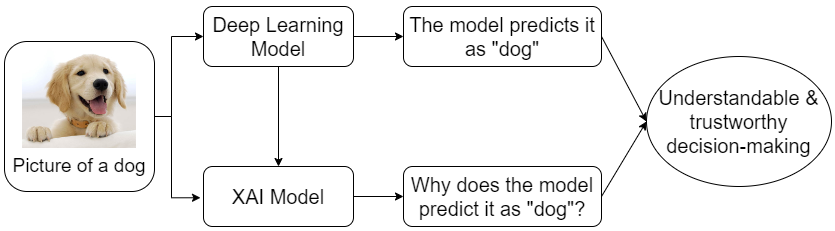
\includegraphics[width=\textwidth]{Images/xai_intro.png}
    \caption[Fundamental way of explaining Deep Learning Models using XAI]{The Schematic represents a fundamental way of getting explanation for a decision made by Deep Learning Models.\cite{XAI_Medical}}
\end{figure}

\begin{table}[h!]
    \centering
    \caption[Importance of Explainability in AI Systems]{Importance of Explainability in AI Systems: Key Needs Addressed by XAI}
    \begin{tabular}{|c|c|}
    \hline
    \textbf{Need} & \textbf{Explanation} \\
    \hline
    Trust & Explainability build trust by showing AI reasoning. \\
    \hline
    Bias Detection & Identifies and addresses biases in AI systems. \\
    \hline
    Compliance & Meets regulatory requirements by explaining decisions. \\
    \hline
    Debugging & Pinpoints issues in AI for improvement. \\
    \hline
    Human-AI Collaboration & Enables better collaboration by understanding AI actions. \\
    \hline
    \end{tabular}
\end{table}

\clearpage

\subsection{Limitations in Common Explainability Methods}

\noindent
Even though there has been a huge amount of work done for interpreting medical images, in which many are attribution methods. The problems with AI method's explainability are:

\begin{itemize}
    \item Attribution methods highlight important areas in an image for CNN Prediction, but not the specific characteristics within the region of focus of the image.
    \item Texture characteristics within the region of activation are not transferred properly, as large parts of image are important for classification.
\end{itemize}

\begin{wrapfigure}{l}{0.5\textwidth}
    \centering
    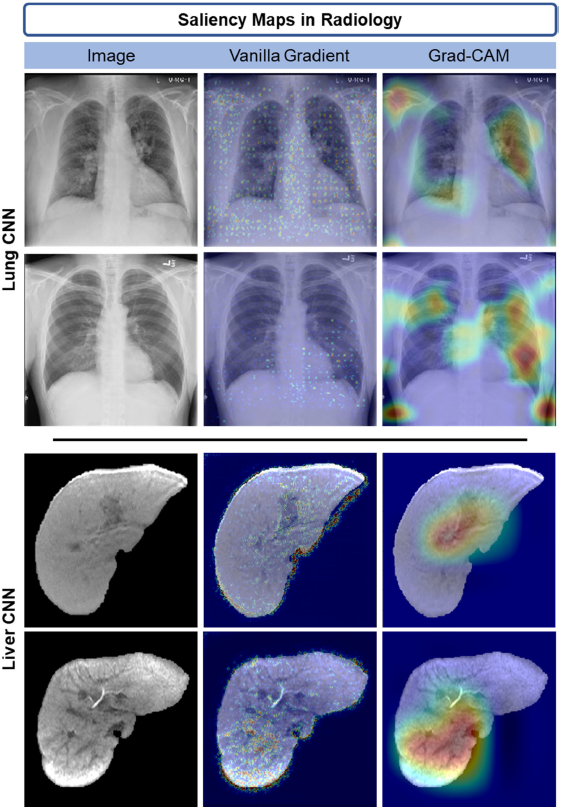
\includegraphics[width=0.5\textwidth]{Images/figan_limitation.png}
    \caption[Limitations of current explainability methods]{Example saliency maps from lung regression and liver classification CNN\cite{FIGAN}}
\end{wrapfigure}

\noindent
The attribution maps in Figure 5.1 highlight attention areas, yet they lack clarity on the specific relevant characteristics within these regions for diagnosis. Within these highlighted areas, various anatomic or texture features could potentially be responsible. In the chest radiograph algorithm, attention might focus on the vasculature, air spaces, or the cardiomediastinal silhouette edge. Similarly, in the liver MRI algorithm, attention might center on hepatic veins, encompassing aspects like the veins themselves, contrast with hepatic parenchyma, or texture.

\noindent
\textit{Attribution: deciding how each feature value in an instance is important in \mbox{obtaining} specific outcomes}

\clearpage

\noindent
For the explainability of AI systems in medical imaging, the 'what' is as likely as important as the 'where'. Current methods provide localization information but their effectiveness is limited in medical imaging, where often multiple objects are spatially co-localized.

\subsection{Other AI Explainability Methods}

\noindent
There are several special methods applied to medical imaging that use CNNs for Explainable AI methods. Some commonly used methods are Attribution Methods and Non-Attribution Methods.

\subsubsection{Attribution Methods}

\noindent
Most explainable AI algorithms are attribution methods, which are a class of algorithms that highlight important areas in an image for a CNN’s prediction. Different types of Attribution Methods are:

\begin{itemize}
    \item Gradient-based Saliency Maps: The most popular form of attribution is gradient-based saliency, which computes the gradient of a prediction with respect to the pixels of the input image\cite{FIGAN}. The visualization of these gradients allows for the interpretation of how input pixels or specific regions impact the CNN's predictions. The gradient-based attribution methods mostly differ in how the gradient is computed. The most popular such methods are Vanilla Gradient maps and Gradient-Weighted Class Activation Mapping

    \item Perturbation-based Saliency Maps: Perturbation maps are another form of saliency that visualize the effect of input feature perturbations on a CNN’s prediction. Perturbed areas of the input image showing a relatively large effect on the CNN predictions are highlighted for interpretation\cite{FIGAN}. Popular approaches are Shapley values and local interpretable model-agnostic explanations.

    \noindent
    Furthermore, while saliency maps effectively highlight clinically significant structures, but interpretation of these can be challenging, particularly in texture and morphology. And these maps are locally interpretable and do not offer a global understanding of CNN's predictive features since they're generated at the image level.
\end{itemize}

\subsubsection{Non-Attribution Methods}

\noindent
Non-attribution methods prioritize the creation of alternative models or explanations without explicitly assigning significance to specific features. Rather than isolating the importance of individual features, these approaches aim to provide a comprehensive understanding of the model's behavior, offering a global view.

\begin{itemize}
    \item Attention Networks
    Attention Networks integrate attention modules directly into the CNN architecture, aiding in both explaining CNN predictions and boosting CNN performance. Rather than employing attribution methods post-training, these modules operate within intermediate CNN layers as feature selectors, amplifying crucial features for prediction and dampening irrelevant ones. Visualizing these augmented feature maps reveals the vital features influencing CNN's predictions. 
    
    \noindent
    However, this approach provides only a localized understanding of the features used for prediction. Attention networks, and CNNs in general, also contain a large number of feature maps within each layer of the network, many of which show little or no activation, making exploration of this feature space less tractable.\cite{FIGAN}
    
    \item Generative Methods
    A novel method to enhance CNN explainability involves creating synthetic images to boost the activation of an output neuron or altering existing images to simulate a different output class. In initial activation maximization techniques, gradient descent was employed to produce an image that maximized a particular neuron's activation, effectively revealing the crucial imaging features influencing a CNN's prediction.
    
    \noindent
    However, the synthetic images produced by these methods do not appear realistic, which makes their interpretation quite difficult, especially in the context of medical images. The proposed model is a GAN-based explainability method that facilitates global interpretation of embedded features important for CNN prediction and shows the resulting embedded feature interpretations that can clarify the ambiguities observed in commonly used attribution maps\cite{FIGAN}.
\end{itemize}

\clearpage

\subsection{Problems Statement}

\noindent
The research in the text addresses the problem of limited explainability in medical imaging classification tasks that use convolutional neural networks (CNNs). While CNNs have shown great performance in these tasks, their complex architectures make it difficult to understand the specific features used by the network to make its decisions. This lack of transparency limits the clinical application of these models and hinders the discovery of new biomarkers for diseases.

\noindent
Current methods for post hoc explainability, such as attribution maps, provide only limited visibility into the characteristics used by CNNs during inference. These methods can highlight areas of attention in an image, but it is not clear what specific characteristics within those areas are relevant to diagnosis. Any of the anatomic or texture characteristics within the highlighted regions could be responsible for CNN's decision. 

\noindent
This problem is particularly relevant for diffuse disease processes where large portions of the image are potentially relevant for classification. For example, in the case of a chest radiograph algorithm designed to infer log NT-pro B-type natriuretic peptide (BNPP) to assess the severity of pulmonary edema, attention could be attributed to any of the following—the vasculature, the interstitium, air spaces. Similarly, for a liver MRI algorithm designed to classify images as having adequate or suboptimal contrast uptake for cancer screening and surveillance to assess the severity of liver fibrosis, attention is centered on hepatic veins but could be attributed to any of the following—the veins themselves, contrast with hepatic parenchyma, or texture. 

\noindent
Therefore, the research proposes a new framework called Feature Interpretation using Generative Adversarial Networks that allows for the dynamic visualization of the features used by a CNN. This framework provides a new level of understanding and explainability in medical imaging classification tasks, improving the transparency of these models for clinical application and potentially uncovering new biomarkers for disease.

\clearpage

\subsection{Proposed Methodology}

\noindent
Generative Adversarial Networks are used in the proposed FIGAN framework to address the problem of limited explainability in medical imaging classification tasks. FIGAN uses CGAN to synthesize images that span the range of CNN's principal embedded features. The GAN is trained to generate images that are similar to the input images but with variations in the specific features of interest. These generated images can then be used to visualize the specific features used by the CNN for classification or regression. 

\noindent
By generating synthetic images that highlight the specific features used by CNN, FIGAN is expected to provide a new level of understanding and explainability in medical imaging classification tasks. 

\noindent
Overall, FIGAN leverages the power of GANs to generate synthetic images that help to clarify ambiguities within attention areas highlighted by existing explainability methods. This approach provides a new tool for interpreting medical imaging-related tasks.

\subsection{FIGAN Architecture}

\noindent
FIGAN is a framework that uses a conditional generative adversarial network to synthesize images that is trained to generate images that are similar to the input images but with variations in the specific features of interest. These generated images can then be used to visualize the specific features used by the CNN for classification or regression.

\noindent
The researchers apply FIGAN to two previously developed CNNs and show that the resulting feature interpretations can clarify ambiguities within attention areas highlighted by existing explainability methods. They also perform a series of experiments to study the effect of auxiliary segmentations, training sample size, and image resolution on FIGAN's ability to provide consistent and interpretable synthetic images.

\noindent
The process (refer to fig 4.3) starts with an input image, and this image is given to a pre-trained CNN, the CNN extracts many features from the input image. These features can be extracted from any intermediate layer within the CNN, but the researchers focused only on the high-level features from the final fully connected layer, which are more likely to explain a CNN’s decisions.

\clearpage

\begin{figure}[h!]
    \centering
    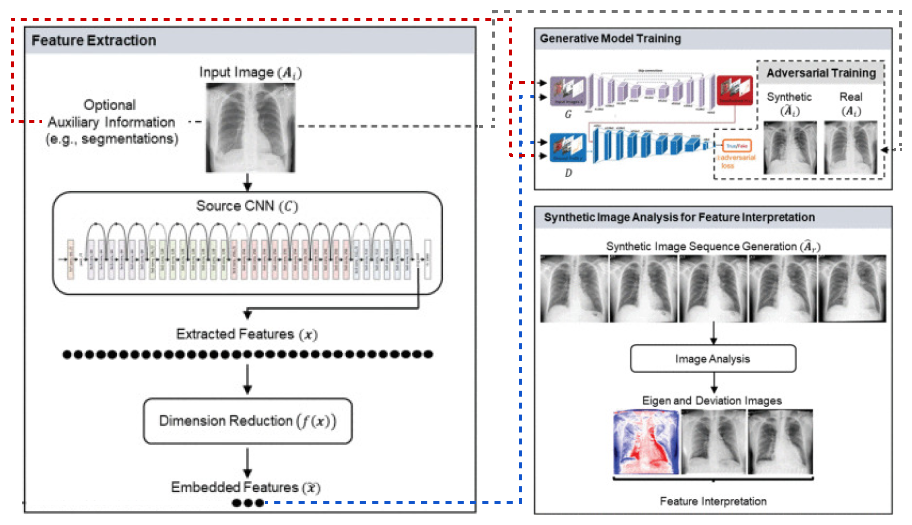
\includegraphics[width=\textwidth]{Images/figan_arch.png}
    \caption{FIGAN Architecture}
\end{figure}

\noindent
As the number of features are more in count, the unwanted features are reduced or deleted using a dimensionality reduction method just like Principal Component Analysis(PCA), but here the researchers have used a method called Partial Least Squares(PLS).

\noindent
\textit{\textbf{PCA}: PCA is an unsupervised technique primarily used for reducing the dimensionality of data while preserving as much variance as possible. It doesn't consider any specific outcome or target variable.}

\noindent
\textit{\textbf{PLS}: PLS is a supervised technique used for dimensionality reduction in the context of regression and predictive modeling. It focuses on finding the directions in the feature space that are most related to the target variable.}

\noindent
The selected features are then given to the CGAN Generator and Discriminator for training the GAN to make realistic images. Now the images made by the CGAN or the synthetic images have most features that actually contribute to CNN's decision-making process, these images are then analyzed, and can be viewed as a Graphics Interchange Format (GIF) or under a medical image viewing device to understand and analyze whether the CNN has taken most relevant features into consideration or not. Thereby getting explainability for the CNN AI system.

\clearpage

\section{Results and Discussion}

\noindent
Understanding the intricate mechanisms within Convolutional Neural Networks has been a long pursuit in computer vision and deep learning. In this section, the focus is directed towards unwind the output produced by the proposed FIGAN Model. This investigation not only promises insights into the inner workings of these models but also holds the potential to utilize these types of AI Systems for visual data analysis in the medical field.

\noindent
The researchers have applied FIGAN to two disease-analyzing CNNs, namely Lung CNN and Liver CNN. They chose three common steps to come up with results from the regenerated images(using FIGAN). They are:

\begin{itemize}

    \item Feature Extraction and Selection
    
    \item Feature Interpretation, and
    
    \item Comparison to Visual Geometry(VG) and Grad-CAM
    
\end{itemize}

\subsubsection{Feature Extraction and Selection}

\noindent
The methodology to get to result was to choose three to five feature maps for regeneration using FIGAN at training steps of 470,000 and the feature map with minimum Fréchet Inception Distance(FID) was chosen for subsequent analysis. And is reported that PLS components have variations in log BNPP. But this result of log BNPP should be interpreted with caution, as Lung and Liver results should be finally interpreted by an expert as per inference table \textit{Applications of explainability in medical imaging\cite{XAI}}.

\noindent
\textit{The Fréchet Inception Distance is a metric used to evaluate the quality of images generated by generative models, especially Generative Adversarial Networks. It measures the similarity between real and generated images by comparing feature representations extracted from a pre-trained Inception network.}

\clearpage

\subsubsection{Feature Interpretation}

\paragraph{Lung CNN Feature Interpretation:}

The authors analyzed the synthetic image sequence and the leading eigen and deviation images for each feature. They found that feature 1 and feature 2 emphasized the importance of cardiomegaly (enlarged heart) and increased perihilar vascularity for predicting log BNPP. Feature 2 also highlighted the importance of the chest wall soft tissues. However, the authors note that feature 3 only explained 1.6\% of variability in log BNPP and must be interpreted with caution.


\paragraph{Liver CNN Feature Interpretation:}

The authors noted that feature 1 emphasized the importance of vessel-liver contrast, which is the primary imaging feature used by radiologists to determine contrast uptake adequacy. Feature 2 highlighted the importance of heterogeneous texture, which is a known correlate of liver pathology. Feature 3 emphasized the importance of liver brightness, which is also a known correlate of liver pathology. The authors note that features 2 and 3 are secondary features of importance for contrast uptake adequacy.

\noindent
\textit{In radiology, "contrast uptake adequacy" refers to the extent or quality of contrast agent absorption or enhancement in a specific organ or tissue region during imaging procedures like CT scans, MRI scans, or other imaging modalities.}

\subsubsection{Comparison to VG and Grad-CAM}

The authors compared the results of using FIGAN to visualize learned features in lung and liver CNN tasks to the results obtained using VG and Grad-CAM. In the lung CNN task, VG showed diffuse network attention scattered throughout the radiograph, while Grad-CAM showed attention toward the left lung and right hilum but could not resolve which structures in these areas drove the regression of NT-proBNP. In contrast, FIGAN images provided insight into variations in heart size and hilar vascular fullness. In the liver CNN task, both VG and Grad-CAM showed attention toward the portal vein, but the meaning of activations scattered throughout the liver was unclear. FIGAN images highlighted liver texture and poor liver vessels, which are associated with inadequate contrast uptake and liver fibrosis.

\clearpage

\noindent
Overall, the results of applying FIGAN to the lung CNN for a regression task provided insights into the imaging features used to predict log BNPP. On the other hand, the results of applying FIGAN to the liver CNN for a classification task provided insights into the imaging features used to determine contrast uptake adequacy. The authors were able to identify primary and secondary imaging features, as well as correlations with the body's physical characteristics of an individual, which may be useful for improving the accuracy and interpretability of medical imaging classification tasks.

\begin{figure}[h!]
    \centering
    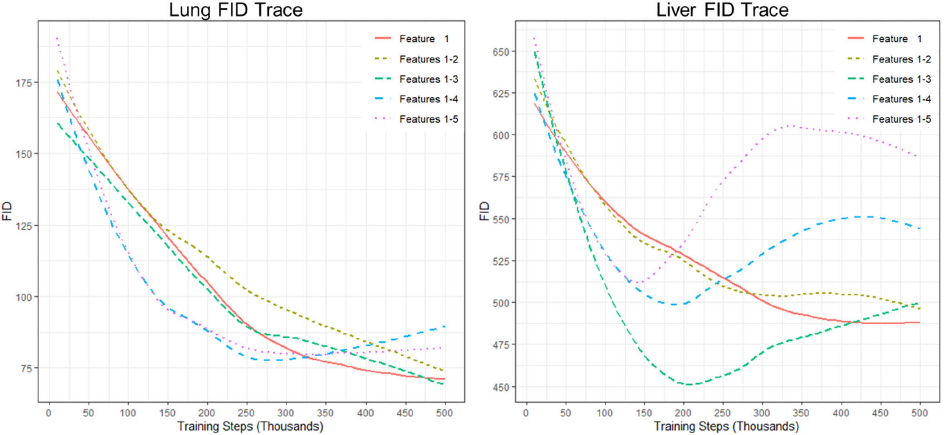
\includegraphics[width=0.9\textwidth]{Images/res_comp_graph.png}
    \caption[Plotted FID traces on applying FIGAN to lung and liver CNNs]{Top three features of Lung CNN shown best FID in FIGAN training. While liver CNN, the first three features.}
\end{figure}

\begin{figure}[h!]
    \centering
    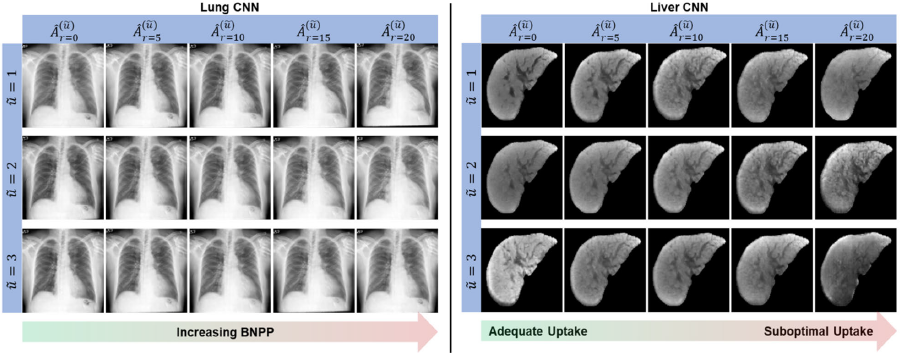
\includegraphics[width=\textwidth]{Images/figan_syn_imgs_seq.png}
    \caption[FIGAN Synthetic Image Sequences]{In chest x-rays, variations emerge in heart size and hilar vascular fullness. While liver MRI shown changes in vessel-liver tissue contrast and liver texture.}
\end{figure}

\clearpage

\section{Applications}

\noindent
The overall work presented in this text has several potential applications in the world of medical imaging and beyond. 

\begin{itemize}
    \item The proposed FIGAN framework provides a new level of understanding and explainability in medical imaging classification tasks. This improved transparency of CNN models can lead to better clinical application of these models and potentially uncover new biomarkers for disease. 
    
    \item Secondly, the use of GANs in FIGAN has broader implications for the field of explainable AI. The ability to generate synthetic images that highlight specific features used by a CNN could be applied to other domains beyond medical imaging, such as natural language processing or computer vision. 

    \item The experiments conducted in this work provide insights into the effect of auxiliary segmentations, training sample size, and image resolution on FIGAN's ability to provide consistent and interpretable synthetic images. These findings could inform the development of future explainability methods and improve the interpretability of CNN models in various domains. 
\end{itemize}

\noindent
Overall, the work presented in this text has the potential to improve the transparency and interpretability of CNN models, leading to better clinical application and potentially uncovering new biomarkers for disease. The use of GANs in FIGAN also has broader implications for the field of explainable AI.

\clearpage

\section{Challenges}

\noindent
The researchers in this text highlight several challenges faced in the field of explainable AI, specifically in the context of medical imaging classification tasks. \\

\noindent
One challenge is the limited explainability of CNN models due to their increasingly complex architectures. While these architectures model highly nonlinear relationships in imaging tasks, they also make it difficult to explain the imaging features used in each image evaluated by the CNN. \\

\noindent
Another challenge is the limited effectiveness of current methods for CNN explainability in medical imaging, where multiple objects are spatially co-localized. Current methods provide localization information, but the relative importance of individual characteristics within the localized region is unknown. \\

\noindent
The researchers also note that existing explainability methods, such as attribution maps, highlight areas of attention but do not clarify what specific characteristics within those areas are relevant to diagnosis. This ambiguity can limit the clinical application of CNN models. \\

\noindent
Overall, the challenges faced by the researchers in this text relate to the limited transparency and interpretability of CNN models in medical imaging classification tasks. These challenges highlight the need for new methods, such as the proposed FIGAN framework, to improve the explainability of CNN models and enable better clinical application.